\documentclass[14pt]{extbook}
\usepackage{multicol, enumerate, enumitem, hyperref, color, soul, setspace, parskip, fancyhdr} %General Packages
\usepackage{amssymb, amsthm, amsmath, latexsym, units, mathtools} %Math Packages
\everymath{\displaystyle} %All math in Display Style
% Packages with additional options
\usepackage[headsep=0.5cm,headheight=12pt, left=1 in,right= 1 in,top= 1 in,bottom= 1 in]{geometry}
\usepackage[usenames,dvipsnames]{xcolor}
\usepackage{dashrule}  % Package to use the command below to create lines between items
\newcommand{\litem}[1]{\item#1\hspace*{-1cm}\rule{\textwidth}{0.4pt}}
\pagestyle{fancy}
\lhead{Makeup Progress Quiz 3}
\chead{}
\rhead{Version A}
\lfoot{1648-1753}
\cfoot{}
\rfoot{Summer C 2021}
\begin{document}

\begin{enumerate}
\litem{
Construct the lowest-degree polynomial given the zeros below. Then, choose the intervals that contain the coefficients of the polynomial in the form $x^3+bx^2+cx+d$.\[ 3 - 2 i \text{ and } -3 \]\begin{enumerate}[label=\Alph*.]
\item \( b \in [1.1, 4], c \in [-5.1, -3.6], \text{ and } d \in [-40, -32] \)
\item \( b \in [-0.4, 2], c \in [-2.9, 0.1], \text{ and } d \in [-9, -4] \)
\item \( b \in [-0.4, 2], c \in [3.2, 8.7], \text{ and } d \in [4, 7] \)
\item \( b \in [-6.7, -1], c \in [-5.1, -3.6], \text{ and } d \in [36, 41] \)
\item \( \text{None of the above.} \)

\end{enumerate} }
\litem{
Describe the end behavior of the polynomial below.\[ f(x) = 2(x - 9)^{3}(x + 9)^{8}(x - 7)^{3}(x + 7)^{5} \]\begin{enumerate}[label=\Alph*.]
\begin{multicols}{2}\item 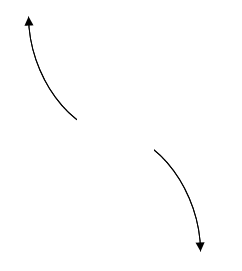
\includegraphics[width = 0.3\textwidth]{../Figures/polyEndBehaviorAA.png}\item 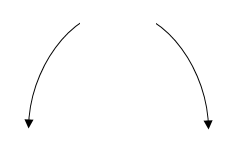
\includegraphics[width = 0.3\textwidth]{../Figures/polyEndBehaviorBA.png}\item 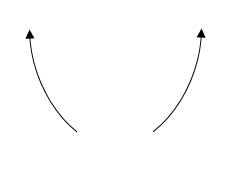
\includegraphics[width = 0.3\textwidth]{../Figures/polyEndBehaviorCA.png}\item 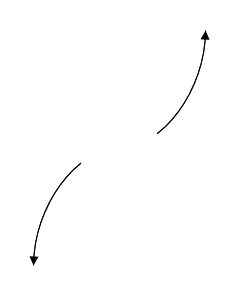
\includegraphics[width = 0.3\textwidth]{../Figures/polyEndBehaviorDA.png}\end{multicols}\item None of the above.
\end{enumerate} }
\litem{
Describe the end behavior of the polynomial below.\[ f(x) = -4(x - 2)^{5}(x + 2)^{10}(x - 3)^{5}(x + 3)^{6} \]\begin{enumerate}[label=\Alph*.]
\begin{multicols}{2}\item 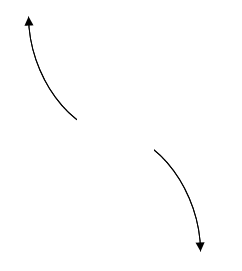
\includegraphics[width = 0.3\textwidth]{../Figures/polyEndBehaviorCopyAA.png}\item 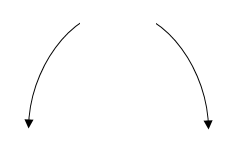
\includegraphics[width = 0.3\textwidth]{../Figures/polyEndBehaviorCopyBA.png}\item 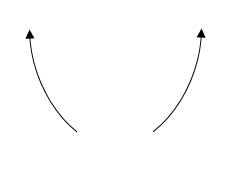
\includegraphics[width = 0.3\textwidth]{../Figures/polyEndBehaviorCopyCA.png}\item 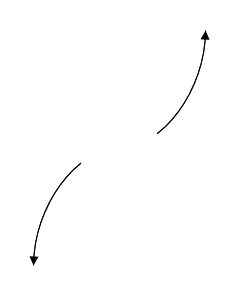
\includegraphics[width = 0.3\textwidth]{../Figures/polyEndBehaviorCopyDA.png}\end{multicols}\item None of the above.
\end{enumerate} }
\litem{
Construct the lowest-degree polynomial given the zeros below. Then, choose the intervals that contain the coefficients of the polynomial in the form $ax^3+bx^2+cx+d$.\[ -6, \frac{-3}{4}, \text{ and } \frac{7}{2} \]\begin{enumerate}[label=\Alph*.]
\item \( a \in [3, 10], b \in [-75, -66], c \in [108, 118], \text{ and } d \in [125, 128] \)
\item \( a \in [3, 10], b \in [-26, -24], c \in [-154, -145], \text{ and } d \in [125, 128] \)
\item \( a \in [3, 10], b \in [23, 33], c \in [-154, -145], \text{ and } d \in [-130, -119] \)
\item \( a \in [3, 10], b \in [-89, -77], c \in [222, 233], \text{ and } d \in [-130, -119] \)
\item \( a \in [3, 10], b \in [23, 33], c \in [-154, -145], \text{ and } d \in [125, 128] \)

\end{enumerate} }
\litem{
Describe the zero behavior of the zero $x = 3$ of the polynomial below.\[ f(x) = 6(x - 3)^{4}(x + 3)^{9}(x + 7)^{4}(x - 7)^{8} \]\begin{enumerate}[label=\Alph*.]
\begin{multicols}{2}\item 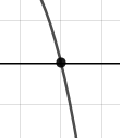
\includegraphics[width = 0.3\textwidth]{../Figures/polyZeroBehaviorAA.png}\item 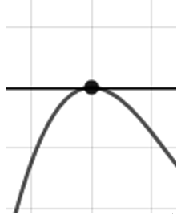
\includegraphics[width = 0.3\textwidth]{../Figures/polyZeroBehaviorBA.png}\item 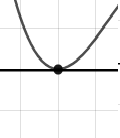
\includegraphics[width = 0.3\textwidth]{../Figures/polyZeroBehaviorCA.png}\item 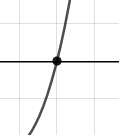
\includegraphics[width = 0.3\textwidth]{../Figures/polyZeroBehaviorDA.png}\end{multicols}\item None of the above.
\end{enumerate} }
\litem{
Which of the following equations \textit{could} be of the graph presented below?
\begin{center}
    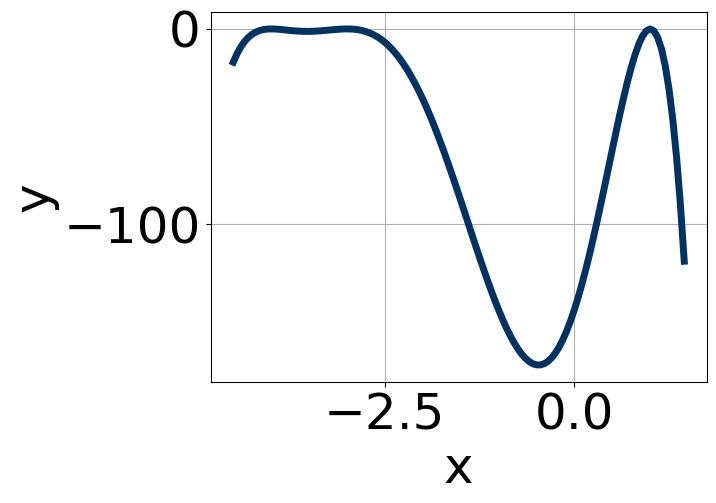
\includegraphics[width=0.5\textwidth]{../Figures/polyGraphToFunctionA.png}
\end{center}
\begin{enumerate}[label=\Alph*.]
\item \( 5x^{5} (x - 3)^{10} (x + 3)^{5} \)
\item \( -7x^{9} (x - 3)^{4} (x + 3)^{9} \)
\item \( -14x^{11} (x - 3)^{5} (x + 3)^{9} \)
\item \( -18x^{9} (x - 3)^{4} (x + 3)^{8} \)
\item \( 17x^{7} (x - 3)^{5} (x + 3)^{5} \)

\end{enumerate} }
\litem{
Construct the lowest-degree polynomial given the zeros below. Then, choose the intervals that contain the coefficients of the polynomial in the form $x^3+bx^2+cx+d$.\[ -2 - 5 i \text{ and } 3 \]\begin{enumerate}[label=\Alph*.]
\item \( b \in [0.2, 3.8], c \in [16.8, 19.7], \text{ and } d \in [-92, -81] \)
\item \( b \in [0.2, 3.8], c \in [-3.5, 0.3], \text{ and } d \in [-9, -3] \)
\item \( b \in [-4.5, 0.5], c \in [16.8, 19.7], \text{ and } d \in [86, 92] \)
\item \( b \in [0.2, 3.8], c \in [1.8, 4.3], \text{ and } d \in [-18, -11] \)
\item \( \text{None of the above.} \)

\end{enumerate} }
\litem{
Describe the zero behavior of the zero $x = 5$ of the polynomial below.\[ f(x) = -9(x - 6)^{11}(x + 6)^{9}(x - 5)^{7}(x + 5)^{6} \]\begin{enumerate}[label=\Alph*.]
\begin{multicols}{2}\item 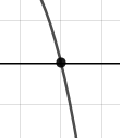
\includegraphics[width = 0.3\textwidth]{../Figures/polyZeroBehaviorCopyAA.png}\item 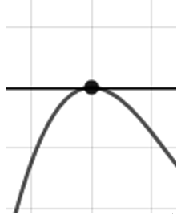
\includegraphics[width = 0.3\textwidth]{../Figures/polyZeroBehaviorCopyBA.png}\item 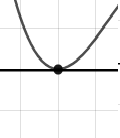
\includegraphics[width = 0.3\textwidth]{../Figures/polyZeroBehaviorCopyCA.png}\item 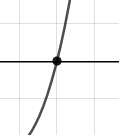
\includegraphics[width = 0.3\textwidth]{../Figures/polyZeroBehaviorCopyDA.png}\end{multicols}\item None of the above.
\end{enumerate} }
\litem{
Construct the lowest-degree polynomial given the zeros below. Then, choose the intervals that contain the coefficients of the polynomial in the form $ax^3+bx^2+cx+d$.\[ \frac{5}{3}, 7, \text{ and } \frac{-7}{5} \]\begin{enumerate}[label=\Alph*.]
\item \( a \in [13, 24], b \in [143, 153], c \in [348, 358], \text{ and } d \in [239, 253] \)
\item \( a \in [13, 24], b \in [-110, -101], c \in [-10, -4], \text{ and } d \in [239, 253] \)
\item \( a \in [13, 24], b \in [-110, -101], c \in [-10, -4], \text{ and } d \in [-247, -238] \)
\item \( a \in [13, 24], b \in [106, 114], c \in [-10, -4], \text{ and } d \in [-247, -238] \)
\item \( a \in [13, 24], b \in [-60, -56], c \in [-287, -277], \text{ and } d \in [-247, -238] \)

\end{enumerate} }
\litem{
Which of the following equations \textit{could} be of the graph presented below?
\begin{center}
    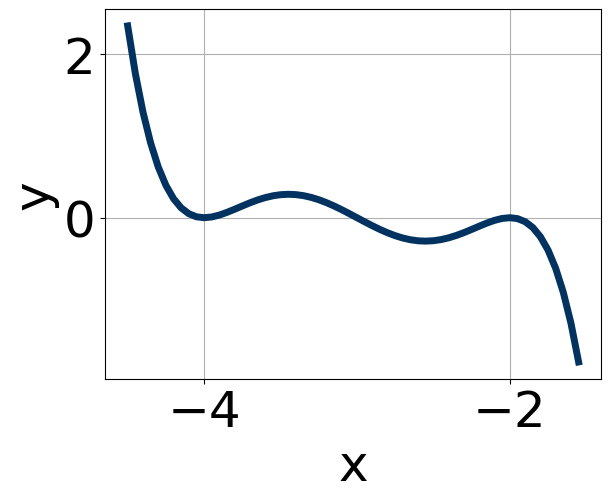
\includegraphics[width=0.5\textwidth]{../Figures/polyGraphToFunctionCopyA.png}
\end{center}
\begin{enumerate}[label=\Alph*.]
\item \( 9x^{4} (x + 3)^{7} (x + 2)^{11} \)
\item \( -20x^{10} (x + 3)^{10} (x + 2)^{11} \)
\item \( 14x^{4} (x + 3)^{9} (x + 2)^{8} \)
\item \( -13x^{9} (x + 3)^{6} (x + 2)^{9} \)
\item \( -18x^{6} (x + 3)^{11} (x + 2)^{9} \)

\end{enumerate} }
\end{enumerate}

\end{document}